% -----------------------------------------------------------------
% Document class: Article
\documentclass[ a4paper, twoside, 11pt]{article}
\usepackage{../../macros-general}
\usepackage{../../macros-article}
% Number of the handout, quiz, exam, etc.
\newcommand{\numero}{02}
\setcounter{numero}{\numero}

% -----------------------------------------------------------------
\begin{document}
\allowdisplaybreaks

\begin{center}
\Large Sistemas de Control (EYAG-1005): Evaluaci\'on \numero \\[1ex]
\small \textbf{Semestre:} 2017-2018 T\'ermino I \qquad
\textbf{Instructor:} Luis Reyes, Jonathan Le\'on
\end{center}
\halfskip

\fbox{

\begin{minipage}[b][\height][t]{\textwidth}
\vspace{0.2 cm}

\begin{center}
\textbf{COMPROMISO DE HONOR}
\end{center}
\vspace{0.4 cm}

\scriptsize
{
Yo, \rule{60mm}{.1pt} al firmar este compromiso, reconozco que la presente evaluaci\'on est\'a dise\~nada para ser resuelta de manera individual, que puedo usar un l\'apiz o pluma y una calculadora cient\'ifica, \linebreak que solo puedo comunicarme con la persona responsable de la recepci\'on de la evaluaci\'on, y que cualquier instrumento de comunicaci\'on que hubiere tra\'ido debo apagarlo. Tambi\'en estoy conciente que no debo consultar libros, notas, \linebreak ni materiales did\'acticos adicionales a los que el instructor entregue durante la evaluaci\'on o autorice a utilizar. Finalmente, me comprometo a desarrollar y presentar mis respuestas de manera clara y ordenada. \\

Firmo al pie del presente compromiso como constancia de haberlo le\'ido y aceptado. 
\vspace{0.4 cm}

Firma: \rule{60mm}{.1pt} \qquad N\'umero de matr\'icula: \rule{40mm}{.1pt} \hspace{0.5cm} \\[-0.8ex]
}

\end{minipage}

}

\vspace{\baselineskip}



% =============================================
\begin{problem} El siguiente Diagrama de Bode muestra la respuesta de la frecuencia de un sistema de segundo orden sub-amortiguado. 

\begin{figure}[htb]
\centering
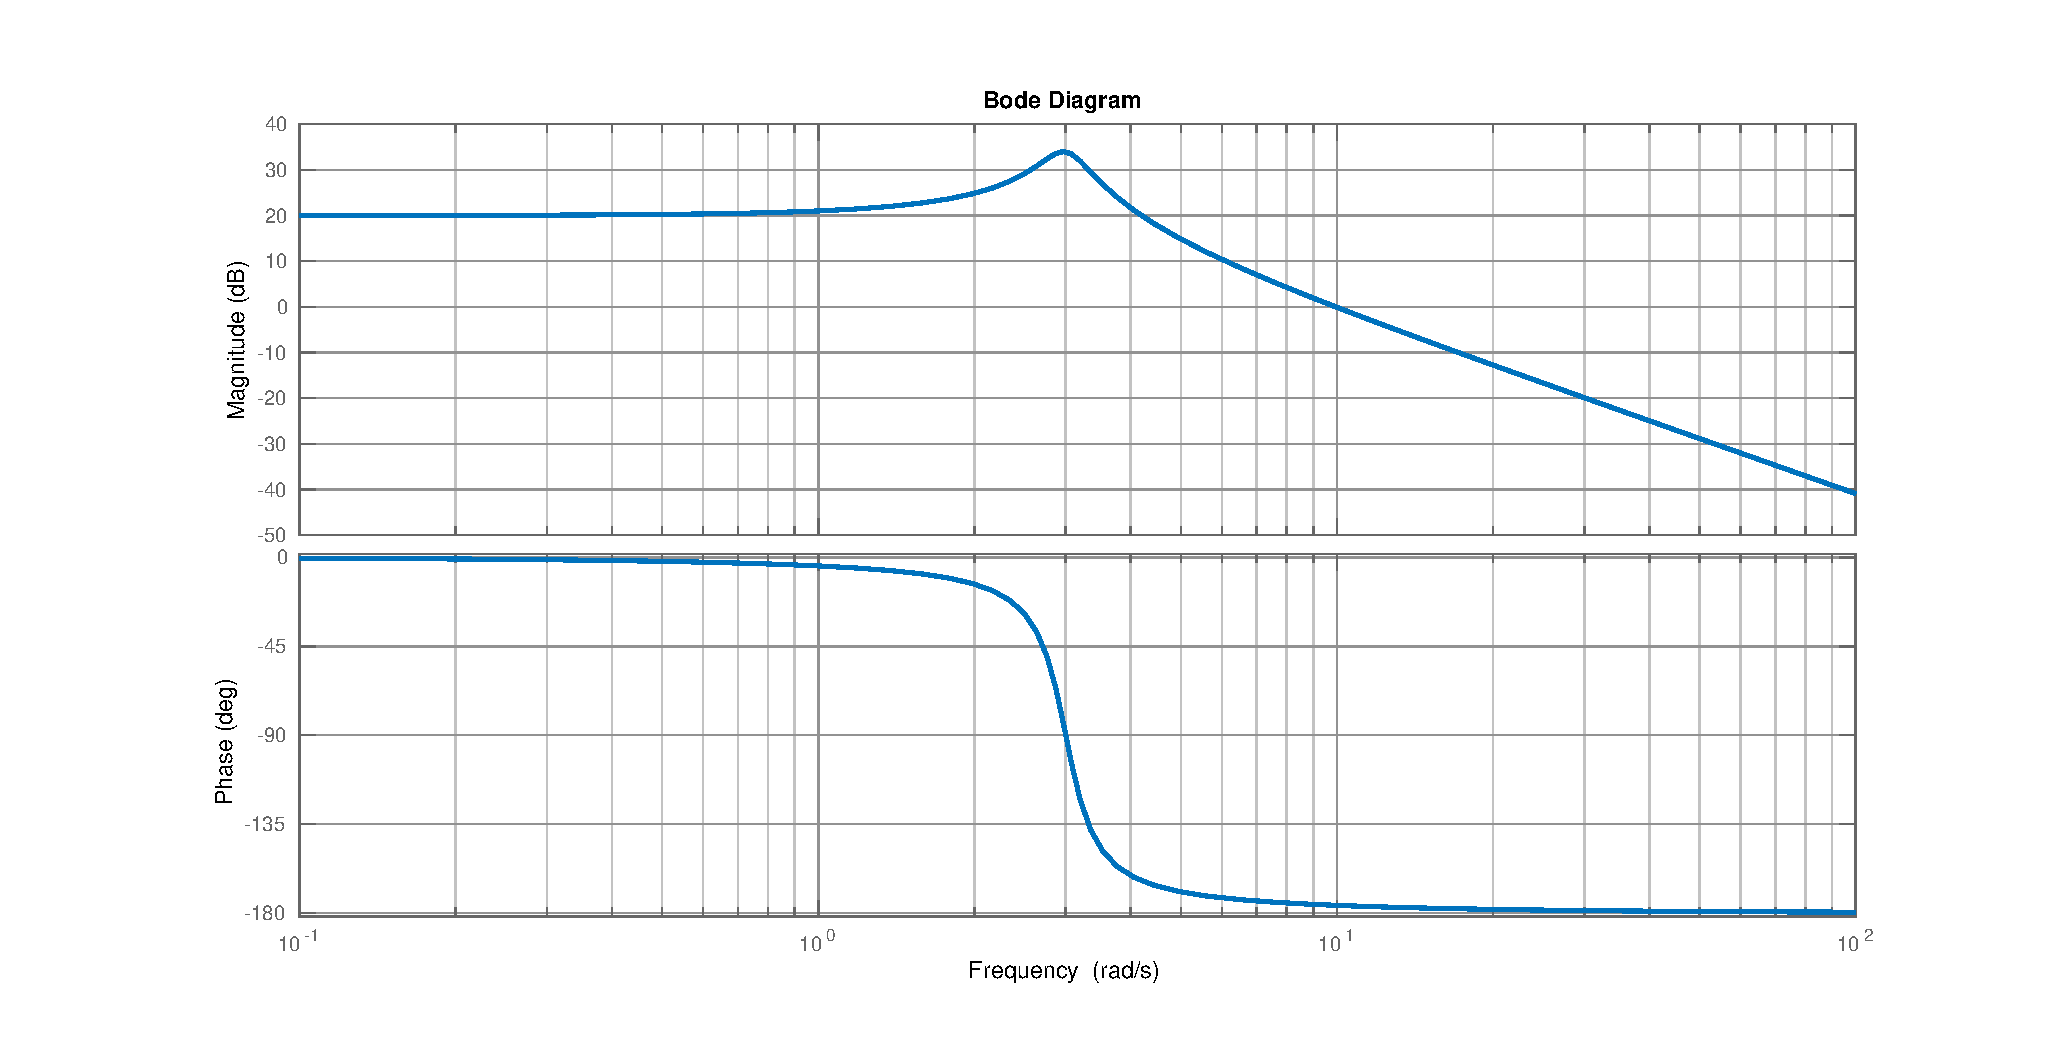
\includegraphics[width=\textwidth]{prob_bode-identificacion.eps}
\end{figure}

Complete las siguientes actividades: 
\begin{itemize}
\item \textbf{[2 Puntos]} Determine la veracidad o falsedad del siguiente enunciado: El margen de ganancia es no mayor a 15 decibeles, \ie $G_M \leq 15 \text{ dB}$. \\ \emph{Soluci\'on:} Falso, el margen de ganancia no existe porque no existe ninguna frecuencia $\omega$ para la cual $\phi(\omega) = -180\deg$. 
\item \textbf{[2 Puntos]} Determine la veracidad o falsedad del siguiente enunciado: El margen de fase es no menor de 40\deg, \ie $\phi_M \geq 40\deg \text{ dB}$. \\ \emph{Soluci\'on:} Falso, pues es claro de la figura que cuando $M(\omega) = 0$ dB es el caso que $\phi(\omega) \leq -160\deg$, lo que implica que $\phi_M \leq 20\deg$. 
\item \textbf{[2 Puntos]} Estime el ancho de banda del sistema. \\ \emph{Soluci\'on:} Dado que la as\'intota de baja frecuencia tiene un valor de 20 dB, para estimar el ancho de banda buscamos la frecuencia $\omega_{BW}$ para la cual $M(\omega_{BW}) = 20 \text{ dB} - 3 \text{ dB} = 17 \text{ dB}$. En particular, $\omega_{BW} \approx 4.5$ rad/s. 
\item \textbf{[4 Puntos]} Encuentre la funci\'on de transferencia del sistema. \\ \emph{Soluci\'on:} Dado que la as\'intota de baja frecuencia tiene un valor de 20 dB, y que la m\'axima magnitud es de 35 dB, reconocemos que la magnitud del pico es de unos 15 dB, \iec
\[
M_p \; = \; 15 \text{ dB} \; = \; 5.62
\]
Adicionalmente: 
\[
M_p \; = \; \frac{1}{ 2 \zeta \, \sqrt{1 - \zeta^2}}
\quad \Longrightarrow \quad
4 \zeta^2 ( 1 - \zeta^2 ) \; = \; M_p^{-1}
\quad \Longrightarrow \quad
\zeta \approx 0.089
\]
Adem\'as, reconociendo que la frecuencia pico $\omega_p \approx 3$ rad/s tenemos que: 
\[
\omega_p \; = \; \omega_n \, \sqrt{1 - 2 \zeta^2}
\quad \Longrightarrow \quad
\omega_n \; = \; \frac{\omega_p}{\sqrt{1 - 2 \zeta^2}}
\; = \; 3.012 \text{ rad/s}
\]
Finalmente, si expresamos la funci\'on de transferencia como
\[
G(s) \; = \; \frac{K}{s^2 + 2 \zeta \omega_n s + \omega_n^2}
\]
entonces para la as\'intota de baja frecuencia tenemos: 
\[
20 \text{ dB} \; = \; 10 \; = \; \frac{K}{\omega_n^2}
\quad \Longrightarrow \quad
K \; = \; 91.44
\]
En conclusi\'on: 
\[
G(s) \; = \; \frac{91.44}{s^2 + 0.536 s + 9.144}
\]

\end{itemize}

\end{problem}
\vspace{\baselineskip}

% =============================================
\begin{problem}
\textbf{[10 Puntos]} Considere el siguiente compensador de atraso de fase: 
\[
G_C(s) \; = \; K \, \frac{(s+z)}{(s+p)} \, ,
\]
Encuentre valores para los par\'ametros $K$, $z$ y $p$ de tal manera que su as\'intota de baja frequencia sea de $+30$ dB, su as\'intota de alta frecuencia sea de $-10$ dB, y su fase sea de $-45\deg$ cuando su frecuencia es de 10 rad/s. 

\emph{Sugerencia:} Para escribir la ecuaci\'on asociada con el \'ultimo requerimiento recuerde que cuando la fase es de $-45\deg$ la parte real de $G( j \omega )$ es igual al negativo de su parte imaginaria. 

\emph{Soluci\'on:} Para la as\'intota de baja frecuencia tenemos: 
\[
\lim_{\omega \rightarrow 0} \, G( j\omega )
\; = \; \frac{K \, z}{p} \; = \; 30 \text{ dB}
\; = \; 31.6 \quad \Longrightarrow \quad
K \, z \; = \; 31.6 \, p
\]
Con respecto a la as\'intota de alta frecuencia, tenemos: 
\begin{align*}
G( j\omega ) \;
& = \; K \, \frac{z + j\omega}{p + j\omega} \cdot \frac{(p-j\omega)}{(p-j\omega)}
\; = \; K \, \frac{(zp + \omega^2) + j \omega (p-z)}{p^2 + \omega^2} \\[2ex]
\Longrightarrow \;
\lim_{\omega \rightarrow \infty} \, G( j\omega ) \;
& = \; \lim_{\omega \rightarrow \infty} \, K \, \frac{(zp + \omega^2) + j \omega (p-z)}{p^2 + \omega^2} \cdot \frac{(1/\omega^2)}{(1/\omega^2)} \; = \; -10 \text{ dB} \; = \; 0.316 \\[2ex]
\Longrightarrow \; K \; & = \; 0.316
\end{align*}
Adicionalmente, para la condici\'on de fase, obtenemos: 
\[
G(10j) \; = \; K \, \frac{(zp + 100) + 10j(p-z)}{p^2 + 100} \quad \Longrightarrow \quad
zp + 100 \; = \; 10(z-p)
\]
Finalmente, combinando las tres ecuaciones anteriores vemos que: 
\[
K \, z \; = \; 31.6 \, p
\quad \Longrightarrow \quad
z = 100 \, p
\quad \Longrightarrow \quad
p \; = \; 0.0102
\]
En conclusi\'on, el compensador debe ser de la forma: 
\[
G_C(s) \; = \; 0.316 \, \frac{(s+1.02)}{(s+0.0102)}
\]

\end{problem}
\vspace{\baselineskip}

% =============================================
\begin{problem} \textbf{[10 Puntos]} Construya un modelo de espacio de estados que represente al mecanismo mostrado en la figura de abajo suponiendo que las salidas son las posiciones de los bloques de masa. 

\begin{figure}[htb]
\centering
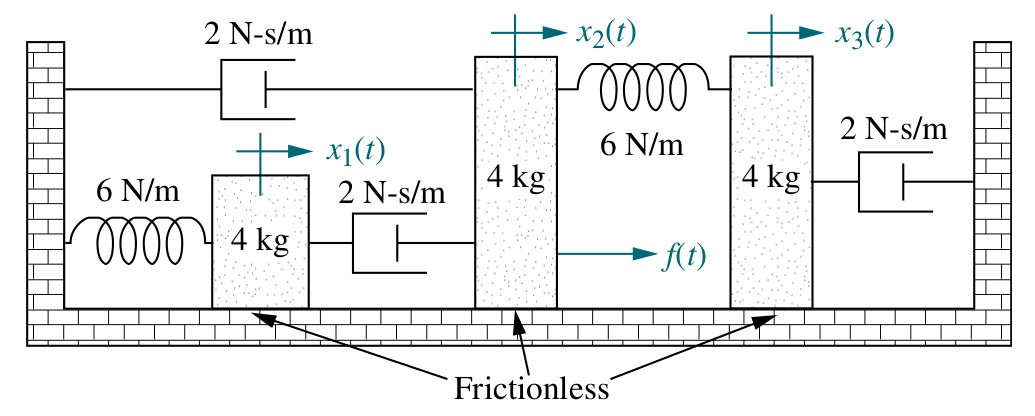
\includegraphics[width=0.68\textwidth]{prob_espacio-estados.jpg}
\end{figure}

\emph{Soluci\'on:} Las ecuaciones de movimiento de los bloques de masa son: 
\begin{align*}
4 \, \ddot{x}_1(t) \;
& = \; -6 \, x_1(t) + 2 \, ( \, \dot{x}_2(t) - \dot{x}_1(t) \, ) \\
4 \, \ddot{x}_2(t) \;
& = \; f(t) -2 \, \dot{x}_2(t) - 2 \, ( \, \dot{x}_2(t) - \dot{x}_1(t) \, ) + 6 \, ( x_3(t) - x_2(t) ) \\
4 \, \ddot{x}_3(t) \;
& = \; -6 \, ( \, x_3(t) - x_2(t) \, ) - 2 \, \dot{x}_3(t)
\end{align*}
Equivalentemente: 
\begin{align*}
\ddot{x}_1(t) \;
& = \; -(3/2) \, x_1(t) - (1/2) \, \dot{x}_1(t) + (1/2) \, \dot{x}_2(t) \\
\ddot{x}_2(t) \;
& = \; +(1/2) \, \dot{x}_1(t) - (3/2) \, x_2(t) - \dot{x}_2(t) + (3/2) \, x_3(t) + (1/4) \, f(t) \\
\ddot{x}_3(t) \;
& = \; +(3/2) \, x_2(t) - (3/2) \, x_3(t) - (1/2) \, \dot{x}_3(t)
\end{align*}
Ahora elegimos la estructura del vector de estado, del vector de entrada y del vector de salida. En nuestro caso: 
\begin{align*}
\vec{x}(t) \;
& = \; (\,
x_1(t), \, \dot{x}_1(t), \,
x_2(t), \, \dot{x}_2(t), \,
x_2(t), \, \dot{x}_3(t) \, ) \\
\vec{u}(t) \;
& = \; f(t) \\
\vec{y}(t) \;
& = \; (\, x_1(t), \, x_2(t), \, x_3(t) \, )
\end{align*}
Entonces nuestras ecuaciones de estado son: 
\[
\vec{\dot{x}}(t) \; = \; 
\left[ \begin{array}{cccccc}
0 & 1 & 0 & 0 & 0 & 0 \\
-(3/2) & -(1/2) & 0 & +(1/2) & 0 & 0 \\
0 & 0 & 0 & 1 & 0 & 0 \\
0 & +(1/2) & -(3/2) & -1 & +(3/2) & +(1/4) \\
0 & 0 & 0 & 0 & 0 & 1 \\
0 & 0 & +(3/2) & 0 & -(3/2) & -(1/2)
\end{array} \right] \, \vec{x}(t) +
\left[ \begin{array}{c}
0 \\ 0 \\ 0 \\ +(1/4) \\ 0 \\ 0
\end{array} \right] \, \vec{u}(t)
\]
Y nuestras ecuaciones de salida son: 
\[
\vec{y}(t) \; = \;
\left[ \begin{array}{cccccc}
1 & 0 & 0 & 0 & 0 & 0 \\
0 & 0 & 1 & 0 & 0 & 0 \\
0 & 0 & 0 & 0 & 1 & 0
\end{array} \right] \, \vec{x}(t) +
\left[ \begin{array}{c}
0
\end{array} \right] \, \vec{u}(t)
\]

\end{problem}
\vspace{\baselineskip}

% =============================================
\begin{problem}
\textbf{[10 Puntos]} Para el siguiente modelo de espacio de estados encuentre la funci\'on de transferencia equivalente. 
\begin{align*}
\vec{\dot{x}}(t) \; & = \; 
\left[ \begin{array}{cc}
-1 & +4 \\ -4 & -1
\end{array} \right] \vec{x}(t) + 
\left[ \begin{array}{c}
+2 \\ -1
\end{array} \right] \vec{u}(t) \\[2ex]
\vec{y}(t) \; & = \; 
\left[ \begin{array}{cc}
1 & 1
\end{array} \right] \vec{x}(t)
\end{align*}

\emph{Soluci\'on:}
\begin{align*}
( \, s \vec{I} - \vec{A} \, )^{-1} \;
& = \; \frac{1}{s^2 + 2s + 17}
\left[ \begin{array}{cc}
s+1 & +4 \\ -4 & s+1
\end{array} \right] \\[2ex]
& \Longrightarrow \; 
( \, s \vec{I} - \vec{A} \, )^{-1} \, \vec{B} \; = \;
\frac{1}{s^2 + 2s + 17}
\left[ \begin{array}{c}
2s - 2 \\ -s - 9
\end{array} \right] \\[2ex]
& \Longrightarrow \; G(s) \; = \;
\vec{C} \, ( \, s \vec{I} - \vec{A} \, )^{-1} \, \vec{B} \; = \;
\frac{s - 11}{s^2 + 2s + 17}
\end{align*}

\end{problem}
\vspace{\baselineskip}

\end{document}
